\documentclass[a4paper,12pt]{article}

\usepackage{amsmath,amssymb,amsthm,tikz}
\usetikzlibrary{calc,arrows.meta}
\usepackage[margin=20mm]{geometry}
\usepackage{hyperref}

\setlength{\parindent}{0pt}
\setlength{\columnsep}{1cm}

\begin{document}

%\twocolumn

\thispagestyle{empty}

\begin{center}
{\Large Assignment 8, 2020-11-09}\\
%{\Large Published on 2020-11-08,}\\
{\em 12 minutes} 
\end{center}

\noindent


\vspace{10pt} 
{\bf Decode Binary Tree to a General One.}\\

Let $a,b,c$ be the last $3$ digits of your Student ID. 
Define a new integer number:
$$N = (a + b) \;\text{mod}\; 10.$$ 

\vspace{5pt}
{\bf (A)} Redraw the binary tree in Figure~\ref{fig:heptagonal-nodes}; 
replace letters $a,b$ with your values. We denote this tree by $B$. 

\vspace{5pt}
{\bf (B)} List all the nodes of $B$ in their in-order DFS traversal order. 

\vspace{5pt} 
{\bf (C)} Draw a general tree (denoted by $G$) that is obtained
by decoding the tree $B$.\\
See \url{https://bit.ly/3kdyg8n} or  
Section 7.3.8, {\em Representing General Trees with Binary Trees}
in the textbook (Goodrich2011, p.309). 

\vspace{5pt} 
{\bf (D)} What is the depth of the node with number $N$ (defined above) in the new tree $G$?




\begin{figure}[!htb]
\center{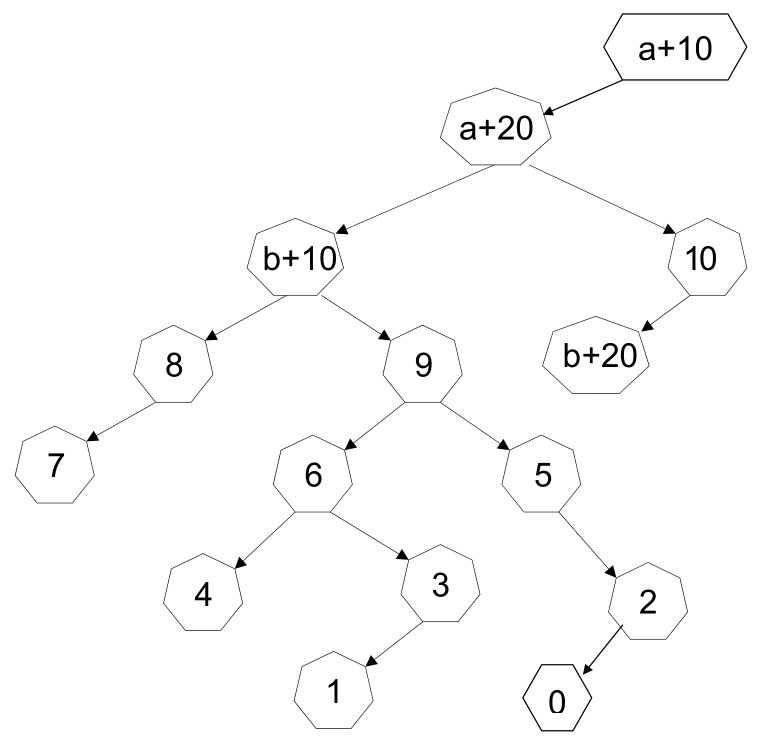
\includegraphics[width=4in]{assignment08-bsts/heptagonal-nodes.png}}
\caption{\label{fig:heptagonal-nodes} Binary tree $B$ to Convert to a General Tree $G$}
\end{figure}








\end{document}



